% !TeX root = orbits.tex

%%%%%%%%%%%%%%%%%%%%%%%%%%%%%%%%%%%%%%%%%%%%%%%%%%%%%%%%%%%%%%%%

\section{Elliptical orbits}\label{s.kepler}

Towards the end of the sixteenth century, the astronomer Tycho Brahe carried out extremely precise observations. In 1600 he hired Johannes Kepler as his assistant and when Tycho died soon afterwards, Kepler was appointed to his position. Here we explain how Kepler was able to establish that planetary orbits are ellipses.

\subsection{Determining the radius of the Earth's orbit}

A Martian year is $687$ days, that is, it equals $\frac{687}{365.25} = 1.88$ Earth years. We know when Mars reaches a new ``year'' by observing its projection on the celestial sphere, but each time the position of the Earth in its orbit will be different. Figure~\ref{f.kepler-mars} shows the orbit of the Earth---its center $O$ offset from the Sun $S$ as Copernicus showed---at four occasions when the position of Mars $M$ at its new year was observed. Four triangles are created $\triangle OE_iM$.

%%%%%%%%%%%%%%%%%%%%%%%%%%%%%%%%%%%%%%%%%%%%%%%%%%%%%%%%%%%%

\begin{figure}[b]
\begin{center}
\begin{tikzpicture}
% The center of the Earth's orbit
\coordinate (O) at (0,0);
\node[below left] at (O) {$O$};

% The circular orbit of the Earth and an arc of the orbit of Mars
\node[draw,circle,minimum size=5cm,name path=Eorbit] at (O) {};
\draw ($(O)+(-35:5)$) arc[start angle=-35,end angle=35,radius=5cm];

% Locate Mars
\coordinate (M) at (-25:5);
\node[right] at (M) {$M$};

% Draw common side OM
\draw[thick] (O) -- (M);

% Locate various positions of the Earth in its orbit
\foreach \angle/\name/\c in { 110/E1/red, 70/E2/purple, 25/E3/{blue}, -40/E4/green} {
  \coordinate (\name) at (\angle:2.5);
  \vertexsmcolor{\name}{\c};
  \draw[\c,thick] (O) -- (\name) -- (M);
}

% Label the Earth's positions
\node[above,yshift=1pt] at (E1) {$E_1$};
\node[above] at (E2) {$E_2$};
\node[right,xshift=2pt] at (E3) {$E_3$};
\node[below,xshift=2pt,yshift=-3pt] at (E4) {$E_4$};

% Nodes drawn at the end to override colors
\vertexsm{M};
\vertexsm{O};

% Draw the Sun
\coordinate (S) at (25:20pt);
\vertexsm{S};
\node[right,yshift=-3pt] at (S) {$S$};

\end{tikzpicture}
\caption{Observations of the orbit of Mars from the Earth}\label{f.kepler-mars}
\end{center}
\end{figure}

%%%%%%%%%%%%%%%%%%%%%%%%%%%%%%%%%%%%%%%%%%%%%%%%%%%%%%%%%%%%

Figure~\ref{f.kepler-one-triangle} shows one of the triangles with the angles labeled. Using the law of sines,
\begin{eqn}
\frac{OE_i}{\sin \beta} &=& \frac{OM}{\sin \alpha}\\[4pt]
OE_i &=& OM\,\frac{\sin \beta}{\sin \alpha}\,.
\end{eqn}

%%%%%%%%%%%%%%%%%%%%%%%%%%%%%%%%%%%%%%%%%%%%%%%%%%%%%%%%%%%%

\begin{figure}[t]
\begin{center}
\begin{tikzpicture}

% The center of the Earth's orbit
\coordinate (O) at (0,0);
\node[below left] at (O) {$O$};

% The circular orbit of the Earth and an arc of the orbit of Mars
\node[draw,circle,minimum size=4cm,name path=Eorbit] at (O) {};
\draw ($(O)+(-45:3.5)$) arc[start angle=-45,end angle=45,radius=3.5cm];

% Locate Mars
\coordinate (M) at (-25:3.5);
\node[right] at (M) {$M$};

% Draw one triangle
\coordinate (E2) at (70:1.75);
\node[above] at (E2) {$E_i$};
\draw[thick] (O) -- (E2) -- (M) -- cycle;

% Label the vertices
\vertexsm{O};
\vertexsm{E2};
\vertexsm{M};
\node[right,xshift=4pt,yshift=3pt] at (O) {$\alpha$};
\node[above left,xshift=-24pt,yshift=14pt] at (M) {$\beta$};
\node[below,xshift=1pt,yshift=-6pt] at (E2) {$\gamma$};

\end{tikzpicture}
\caption{One triangle Earth-Sun-Moon}\label{f.kepler-one-triangle}
\end{center}
\end{figure}

%%%%%%%%%%%%%%%%%%%%%%%%%%%%%%%%%%%%%%%%%%%%%%%%%%%%%%%%%%%%

\begin{table}[b]
\[
\begin{array}{rrrrr}
\hline
& \multicolumn{1}{c}{\alpha} & \multicolumn{1}{c}{\beta} &
  \multicolumn{1}{c}{\gamma} & \multicolumn{1}{c}{OE_i \,\scriptstyle(\times OM)} \\\hline
E_1 & 127.1 & 20.8  & 32.1 & 0.6682\\
E_2 & 84.2 & 35.8 & 60.5 & 0.6721\\
E_3 & 41.3 & 42.4 &96.4 & 0.6785\\
E_4 & 1.6& 3.4& 175.0 & 0.6805\\
\hline
\end{array}
\]
\caption{Tycho's measurements of the distance of the Earth from the center}\label{tab.tycho}
\end{table}

%%%%%%%%%%%%%%%%%%%%%%%%%%%%%%%%%%%%%%%%%%%%%%%%%%%%%%%%%%%%

Tycho Brahe was able to measure all three angles (Table~\ref{tab.tycho})\footnote{The values are rounded to one decimal point.}. The values of $OE$ are given in the fourth column of the table and they are not equal. Assuming (as everyone did at that time) that the Earth' orbit is circular, the only solution was to move the center of the orbit so that $\{E_1,E_2,E_3,E_4\}$ were all on the circle.

\subsection{Measuring the angles in the triangle Sun-Earth-Mars}

How can the angles $\alpha, \beta, \gamma$ be measured? Since $\triangle E_iOM$ is a triangle, it is sufficient to measure two of the angles. $\gamma$ is easily measured by observing Mars and the Sun at the same time. However, neither $\alpha$ nor $\beta$ can be measured directly since they are not accessible to an observer on Earth.

Tycho's measurement used the known periods of the orbits to compute the angles. The Earth moves counterclockwise around Sun. Given any point $E$, after $t$ days the Earth will eventually move to $E'$ and Mars will move to $M'$ so that they are in \emph{opposition}, that is, Mars will be in the continuation of the Earth-Sun line (Figure~\ref{f.kepler-opposition}). Since the Earth completes an orbit in close to half the time that Mars takes, this will occur before either has completed a full orbit. The angles $\theta_E$ and $\theta_M$ are fractions of a circular orbit of $360^\circ$, so
\begin{eqn}
\frac{t}{365.25} &=& \frac{\theta_E}{360}\\[4pt]
\theta_E &=& \frac{360\,t}{365.35}\\[4pt]
\frac{t}{687} &=& \frac{\theta_M}{360}\\[4pt]
\theta_M &=& \frac{360\,t}{687}\,.
\end{eqn}
This gives values for $\theta_E$ and $\theta_M$. From geometry we have
\begin{eqn}
\alpha' &=& 180-\theta_E = \alpha-\theta_M\\
\alpha &=& 180 - \theta_E + \theta_M\,,
\end{eqn}
and the values of $OE_i$ in Table~\ref{tab.tycho} can be computed.

%%%%%%%%%%%%%%%%%%%%%%%%%%%%%%%%%%%%%%%%%%%%%%%%%%%%%%%%%%%%

\begin{figure}[t]
\begin{center}
\begin{tikzpicture}

% The center of the Earth's orbit
\coordinate (O) at (0,0);
\node[below] at (O) {$O$};

% The circular orbit of the Earth and an arc of the orbit of Mars
\node[draw,circle,minimum size=4cm,name path=Eorbit] at (O) {};
\draw ($(O)+(-45:3.5)$) arc[start angle=-45,end angle=45,radius=3.5cm];

% Locate Mars
\coordinate (M) at (-25:3.5);
\node[right] at (M) {$M$};

% Draw one triangle
\coordinate (E2) at (70:1.75);
\node[above] at (E2) {$E$};
\draw (O) -- (E2) -- (M) -- cycle;

\vertexsm{O};
\vertexsm{E2};
\vertexsm{M};

\node[right,xshift=8pt,yshift=20pt] at (O) {$\alpha'$};
\node[above left,xshift=-24pt,yshift=14pt] at (M) {$\beta$};
\node[below,xshift=1pt,yshift=-6pt] at (E2) {$\gamma$};

\draw ($(O)+(-25:.5)$) arc[start angle=-25,end angle=20,radius=.5cm];
\node[right,xshift=12pt,yshift=-1pt] at (O) {$\theta_M$};
\draw ($(O)+(20:.5)$) arc[start angle=20,end angle=70,radius=.5cm];
\node[right,xshift=12pt,yshift=-1pt] at (O) {$\theta_M$};
\draw ($(O)+(70:.5)$) arc[start angle=70,end angle=200,radius=.5cm];
\node[above left,xshift=-4pt,yshift=10pt] at (O) {$\theta_E$};


\coordinate (E2P) at (200:2);
\vertexsm{E2P};
\node[left] at (E2P) {$E'$};
\coordinate (MPP) at (20:4);
\vertexsm{MPP};
\node[above right] at (MPP) {$M'$};
\draw[thick] (E2P) -- (MPP);

\end{tikzpicture}
\caption{The Earth and Mars in opposition}\label{f.kepler-opposition}
\end{center}
\end{figure}

%%%%%%%%%%%%%%%%%%%%%%%%%%%%%%%%%%%%%%%%%%%%%%%%%%%%%%%%%%%%

\subsection{A new location for the center of the Earth's orbit}

Kepler's next task was to obtain a new value $O'$ for the center of the Earth's orbit such that the $E_i$ in Table~\ref{tab.tycho} are on the orbit. We need the following theorem in geometry.

\begin{theorem}\label{thm.three-points}
Given three non-collinear points,\footnote{\emph{Collinear} means that the points all on the same line.} a circle can be constructed that goes through all three points.
\end{theorem}

\begin{proof}
Three non-collinear points $A,B,C$ define a triangle $\triangle ABC$ (Figure~\ref{f.kepler-circumscribed}). Construct the perpendicular bisectors of any two of its three sides, say, $AC$ and $BC$. By definition the perpendicular bisector is the geometric locus of points equidistant from the endpoints of the segment. Let $O$ be the intersection of the two bisectors. Then the $AO=CO=BO$ is the radius of a circle centered at $O$ that goes through $A,B,C$.\hqed
\end{proof}

\begin{figure}
\begin{center}
\begin{tikzpicture}[scale=.8]
  % Define the coordinates of an arbitrary triangle,
  %   label the vertices and draw dots at each vertex
  \coordinate[label = left:$A$]  (A) at ( 0, 0);
  \coordinate[label = right:$B$] (B) at (5, 0);
  \coordinate[label = above:$C$] (C) at (3.5 ,4);
  \vertexsm{A};
  \vertexsm{B};
  \vertexsm{C};
  
  % Draw the triangle
  \draw (A) -- (B) -- (C) -- cycle;

  % Construct perpendicular bisectors
  \coordinate (AC) at ($(A)!.5!(C)$);
  \draw[name path=ac] ($(AC)!1.5cm!-90:(A)$) -- ($(AC)!2.5cm!90:(A)$);
  \coordinate (BC) at ($(B)!.5!(C)$);
  \draw[name path=bc] ($(BC)!3cm!-90:(B)$) -- ($(BC)!.5cm!90:(B)$);

  % Find the intersection
  \path [name intersections = {of = bc and ac, by = {M}}];
  \vertexsm{M};
  \node[above right,xshift=-1pt,yshift=2pt] at (M) {$O$};

  % Construct a circumscribed circle
  \node[draw] at (M) [circle through = (A)] {};

  \draw[rotate=-40] (AC) rectangle +(6pt,6pt);
  \draw[rotate=200] (BC) rectangle +(6pt,6pt);

\end{tikzpicture}
\caption{A circle through three arbitrary points}\label{f.kepler-circumscribed}
\end{center}
\end{figure}

%%%%%%%%%%%%%%%%%%%%%%%%%%%%%%%%%%%%%%%%%%%%%%%%%%%%%%%%%%%%

Given the new locations of the Earth $\{E_1,E_2,E_3,E_4\}$, a circle centered at $O'$ can be constructed that goes through $\{E_1,E_2,E_3\}$ (Figure~\ref{f.kepler-earth-new}). To verify that this is the correct orbit, check that $E_4$ is on the circle.

%%%%%%%%%%%%%%%%%%%%%%%%%%%%%%%%%%%%%%%%%%%%%%%%%%%%%%%%%%%%

\begin{figure}[b]
\begin{center}
\begin{tikzpicture}

% The center of the Earth's orbit
\coordinate (O) at (0,0);
\vertexsm{O};
\node[below left] at (O) {$O$};

% The circular orbit of the Earth and an arc of the orbit of Mars
\node[draw,circle,minimum size=5cm,name path=Eorbit] at (O) {};
\draw ($(O)+(-35:5)$) arc[start angle=-35,end angle=35,radius=5cm];

% Locate Mars
\coordinate (M) at (-25:5);
\node[right] at (M) {$M$};

% Draw the Sun
\coordinate (S) at (25:30pt);
\vertexsm{S};
\node[right,yshift=-3pt] at (S) {$S$};

% Draw the center of the new orbit
\coordinate (OP) at (25:12pt);
\vertexsm{OP};
\node[below,yshift=-2pt] at (OP) {$O'$};
\draw (O) -- (OP);

% Draw new orbit
\node[draw,thick,dashed,circle,minimum size=5cm,
      name path=Eorbitnew] at (OP) {};

% Draw common side OM
\draw[thick] (OP) -- (M);

% Locate various positions of the Earth in its orbit
\foreach \angle/\name/\c in { 110/E1/red, 70/E2/purple, 25/E3/{blue}, -40/E4/green} {
  \coordinate (\name) at ($(OP)+(\angle:2.5)$);
  \vertexsmcolor{\name}{\c};
  \draw[\c,thick] (OP) -- (\name) -- (M);
}

% Label the Earth's positions
\node[above left,yshift=1pt] at (E1) {$E_1$};
\node[above right] at (E2) {$E_2$};
\node[right,xshift=2pt] at (E3) {$E_3$};
\node[below,xshift=2pt,yshift=-3pt] at (E4) {$E_4$};

% Nodes drawn at the end to override colors
\vertexsm{M};
\vertexsm{OP};

\end{tikzpicture}
\caption{Observations of the orbit of Mars from the new Earth's orbit}\label{f.kepler-earth-new}
\end{center}
\end{figure}

%%%%%%%%%%%%%%%%%%%%%%%%%%%%%%%%%%%%%%%%%%%%%%%%%%%%%%%%%%%%

\subsection{Orbits are ellipses}

While Kepler was able to modify the center of the orbit of the Earth to be consistent with the observations, he was not able to adequately describe the orbit of Mars. After years of work, he came to the conclusion that the orbit must be oval like an egg. Oval, perhaps, but certainly not an ellipse, because he was certain that it would have been discovered by Archimedes! Figure~\ref{f.kepler-egg} shows $C$, a position on a circular orbit, and an oval orbit (dashed), where $M$ is the position of Mars on the oval corresponding to $C$. The radius of the circular orbit is labeled $a$ and the unknown distances to $M$ are labeled $s=SM$ and $t=OM$.

Kepler's computed that $\displaystyle\frac{a-t}{t} = 0.00429$ and $\displaystyle\frac{s}{t} = 1.00429$, so that
\begin{eqn}
\frac{a-t}{t} &=& \frac{s}{t}-1\\
a-t &=& s=t\,,
\end{eqn}
and therefore $SM=s=a=AO=CO$. If the dashed oval is, in fact, an ellipse, because in an ellipse $SM=AO$ (by Theorem~\ref{thm.ellipses-features}). Kepler then computed the projections of the observations of Mars on the $x$-axis (Figure~\ref{f.kepler-ellipse}) and obtained for all of them that
\[
\frac{M_iO_i}{C_iO_i} = \frac{1}{1.00429}=0.99573\,.
\]
By Theorem~\ref{thm.ellipse-b-over-a}, since the ratio $MO/CO=b/a$ is constant for in an ellipse, Kepler was able to conclude that the orbit of Mars is an ellipse.

%%%%%%%%%%%%%%%%%%%%%%%%%%%%%%%%%%%%%%%%%%%%%%%%%%%%%%%%%%%%

\begin{figure}[t]
\begin{center}
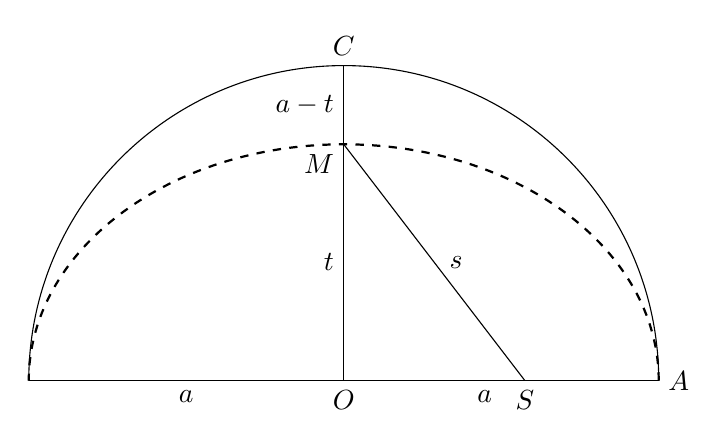
\begin{tikzpicture}
% The center of the Earth's orbit
\coordinate (O) at (0,0);
\node[below] at (O) {$O$};
\vertexsm{O};
\coordinate (C) at (0,4);
\coordinate (A) at (4,0);

% The circular orbit of the Earth and an elliptical orbit of Mars
\draw[thick,dashed] (A) arc(0:180:4cm and 3cm);
\draw (4,0) arc(0:180:4cm);
\draw (0,0) -- (C) node[above] {$C$};
\draw (-4,0) -- node[below] {$a$} (O) -- 
  node[below,xshift=-6pt] {$a$} (A) node[right] {$A$};

% Locate Mars
\coordinate (M) at (0,3);
\node[below left] at (M) {$M$};
\vertexsm{M};

% Locate the Sun
\coordinate (S) at (2.3,0);
\vertexsm{S};
\node[below] at (S) {$S$};

% Draw line from Sun to Mars
\draw (M) -- node[right,xshift=2pt] {$s$} (S);
\path (O) -- node[left] {$t$} (M) -- node[left] {$a-t$} (C);

\end{tikzpicture}
\caption{The orbit of Mars as an oval ``egg''}\label{f.kepler-egg}
\end{center}
\end{figure}

%%%%%%%%%%%%%%%%%%%%%%%%%%%%%%%%%%%%%%%%%%%%%%%%%%%%%%%%%%%%

\begin{figure}[b]
\begin{center}
\begin{tikzpicture}
% The center of the Earth's orbit
\coordinate (O) at (0,0);
\node[below] at (O) {$O$};
\vertexsm{O};

% The circular orbit of the Earth and an elliptical orbit of Mars
\draw[thick,dashed,name path=ellipse] (4,0) arc(0:180:4cm and 3cm);
\draw[name path=circle] (4,0) arc(0:180:4cm);
\draw (0,0) -- (0,4) node[above] {$C$};
\draw (-4,0) -- (4,0); % node[right] {$A$};

% Locate Mars
\coordinate (M) at (0,3);
\node[below left] at (M) {$M$};
\vertexsm{M};

% Locate the Sun
\coordinate (S) at (2.8,0);
\vertexsm{S};
\node[below] at (S) {$S$};

% Locate the projections
\coordinate (O1) at (-3,0);
\node[below] at (O1) {$O_1$};
\coordinate (O2) at (-1,0);
\node[below] at (O2) {$O_2$};
\coordinate (O3) at (1.8,0);
\node[below] at (O3) {$O_3$};

% Get intersections with the circle
\path[name path=P1] (O1) -- +(0,4.2);
\path[name path=P2] (O2) -- +(0,4.2);
\path[name path=P3] (O3) -- +(0,4.2);

\path [name intersections = {of = circle and P1, by = {C1} }];
\path [name intersections = {of = circle and P2, by = {C2} }];
\path [name intersections = {of = circle and P3, by = {C3} }];

% Get intersections with the ellipse
\path [name intersections = {of = ellipse and P1, by = {M1} }];
\path [name intersections = {of = ellipse and P2, by = {M2} }];
\path [name intersections = {of = ellipse and P3, by = {M3} }];

\draw (O1) -- (C1) node[above,yshift=4pt] {$C_1$};
\draw (O2) -- (C2) node[above] {$C_2$};
\draw (O3) -- (C3) node[above] {$C_3$};

% Label positions of Mars on the ellipse
\vertexsm{M1} node[below right] {$M_1$};
\vertexsm{M2} node[below left,yshift=-4pt,xshift=1pt] {$M_2$};
\vertexsm{M3} node[below left] {$M_3$};

\end{tikzpicture}
\caption{The orbit of Mars as an ellipse}\label{f.kepler-ellipse}
\end{center}
\end{figure}
